\documentclass[11pt,letterpaper]{article}

\usepackage[utf8]{inputenc}
\usepackage[T1]{fontenc}
\usepackage[spanish,es-nodecimaldot]{babel}
\usepackage{lmodern}
\usepackage{geometry}
\usepackage{xcolor}
\usepackage{graphicx}
\usepackage{amsmath}
\usepackage{booktabs}
\usepackage{tabularx}
\usepackage{longtable}
\usepackage{array}
\usepackage{enumitem}
\usepackage{fancyhdr}
\usepackage{hyperref}
\usepackage{url}
\usepackage{microtype}
\usepackage{lastpage}

\geometry{top=2.2cm,bottom=2.3cm,left=2.2cm,right=2.2cm}
\setlength{\parindent}{0pt}
\setlength{\parskip}{6pt}
\setlength{\headheight}{14pt}
\setlist[itemize]{leftmargin=1.4em,itemsep=2pt,topsep=3pt}
\setlist[enumerate]{leftmargin=1.6em,itemsep=2pt,topsep=3pt}
\renewcommand{\arraystretch}{1.22}
\emergencystretch=2em

\definecolor{utbblue}{HTML}{003A70}
\definecolor{utbmid}{HTML}{005B96}
\definecolor{utborange}{HTML}{F28C28}
\definecolor{ink}{HTML}{17212B}
\definecolor{muted}{HTML}{5C6773}
\definecolor{softblue}{HTML}{EAF3F8}
\definecolor{softorange}{HTML}{FFF3E6}
\definecolor{softgray}{HTML}{F3F5F7}
\definecolor{success}{HTML}{18794E}
\definecolor{warning}{HTML}{9A5B00}

\hypersetup{
  colorlinks=true,
  linkcolor=utbblue,
  urlcolor=utbmid,
  pdftitle={Evaluación del proyecto UTB Te acompaña},
  pdfauthor={Emmanuel Ascendra Pérez},
  pdfsubject={Reto IA Bolívar 2026}
}

\pagestyle{fancy}
\fancyhf{}
\lhead{\textcolor{utbblue}{\textbf{UTB Te acompaña}}}
\rhead{\textcolor{muted}{Evaluación del proyecto}}
\cfoot{\textcolor{muted}{Página \thepage\ de \pageref*{LastPage}}}
\renewcommand{\headrulewidth}{0.4pt}

\newcommand{\taglabel}[2]{%
  \noindent\colorbox{#1}{\parbox{\dimexpr\linewidth-2\fboxsep\relax}{\textcolor{white}{\textbf{#2}}}}\par
}

\newcommand{\evidencebox}[1]{%
  \noindent\fcolorbox{utbmid}{softblue}{%
    \parbox{\dimexpr\linewidth-2\fboxsep-2\fboxrule\relax}{%
      \textcolor{utbblue}{\textbf{Evidencia verificable.}} #1
    }%
  }\par
}

\newcommand{\caveatbox}[1]{%
  \noindent\fcolorbox{utborange}{softorange}{%
    \parbox{\dimexpr\linewidth-2\fboxsep-2\fboxrule\relax}{%
      \textcolor{warning}{\textbf{Alcance y cautela.}} #1
    }%
  }\par
}

\newcommand{\proposalbox}[1]{%
  \noindent\fcolorbox{muted}{softgray}{%
    \parbox{\dimexpr\linewidth-2\fboxsep-2\fboxrule\relax}{%
      \textcolor{ink}{\textbf{Propuesta pendiente de validación institucional.}} #1
    }%
  }\par
}

\newcommand{\question}[3]{%
  \section{#1}
  \taglabel{#2}{#3}
}

\begin{document}
\hypersetup{pageanchor=false}

\begin{titlepage}
  \thispagestyle{empty}
  \centering
  \vspace*{0.7cm}
  
\includegraphics[width=0.28\textwidth]{../apps/web/public/front/utb-logo.png}

  \vspace{1.2cm}
  {\color{utbblue}\rule{\textwidth}{2.2pt}}
  \vspace{0.8cm}

  {\Huge\bfseries\color{utbblue} UTB Te acompaña\par}
  \vspace{0.35cm}
  {\LARGE\bfseries Informe de evaluación del proyecto\par}
  \vspace{0.3cm}
  {\large Alineación, retorno, implementación, datos, ética y adopción\par}

  \vspace{1.0cm}
  \fcolorbox{utborange}{softorange}{%
    \parbox{0.82\textwidth}{\centering
      \textbf{Reto IA Bolívar 2026}\\[2mm]
      Plataforma de acompañamiento estudiantil y prevención de la deserción \\
      Pagina Web: \url{https://reto-ia-bolivar.vercel.app/} \\
      Repositorio: \url{https://github.com/GhostAnalyst30}
    }%
  }

  \vfill
  \begin{tabular}{rl}
    \textbf{Desarrolladores:} & Emmanuel Ascendra Pérez\\[2mm]
    \textbf{Institución:}     & Universidad Tecnológica de Bolívar\\
    \textbf{Fecha:}           & 29 de julio de 2026\\
  \end{tabular}

  \vfill
\end{titlepage}

\hypersetup{pageanchor=true}
\pagenumbering{roman}
\tableofcontents
\newpage
\pagenumbering{arabic}

\section*{Resumen ejecutivo}
\addcontentsline{toc}{section}{Resumen ejecutivo}

\textbf{UTB Te acompaña} es un MVP avanzado de acompañamiento estudiantil para la
Universidad Tecnológica de Bolívar. Su objetivo es convertir señales dispersas
---actividad, caracterización, progreso, estado de ánimo y solicitudes de apoyo---
en alertas explicables y casos priorizados para que Bienestar Universitario pueda
intervenir antes de que el riesgo de deserción se materialice.

El prototipo integra un portal estudiantil, Digital Twin determinístico, chat de
acompañamiento con guardrails, orientación vocacional, motor de riesgo, CareQueue,
agendamiento con psicología y tableros institucionales. La arquitectura usa
Next.js, FastAPI, Supabase/PostgreSQL y proveedores LLM en cascada. El núcleo de
riesgo es auditable: cada puntaje conserva factores, pesos, causa dominante y
fecha de cálculo. Los casos críticos se transfieren a personal humano.

\begin{center}
\begin{tabularx}{\textwidth}{>{\bfseries\color{utbblue}}p{0.23\textwidth} X}
\toprule
Estado & Prototipo funcional con componentes productivos y otros aún en modo demo o scaffold.\\
Datos & Seeds y cuentas ficticias para demostración; no existe dataset ERP real versionado.\\
Validación & 35 pruebas unitarias definidas en tres módulos; CI valida TypeScript, build web e import del API.\\
Modelo & Riesgo heurístico operativo; regresión logística opcional, sin artefacto entrenado versionado.\\
ROI & Escenario conservador estimado: 116\% en el primer año, sujeto a validación mediante piloto.\\
Gobernanza & Controles técnicos implementados; validación jurídica, dueño formal y plan de adopción están pendientes.\\
\bottomrule
\end{tabularx}
\end{center}

\caveatbox{Los indicadores de retención, matrícula y satisfacción presentes en
la landing y en los seeds son datos de demostración. Este informe no los utiliza
como resultados de impacto real. Del mismo modo, las cifras financieras son un
escenario de planeación, no costos contables ni beneficios ya realizados.}

\section*{Método y criterio de evidencia}
\addcontentsline{toc}{section}{Método y criterio de evidencia}

El análisis distingue tres niveles:
\begin{itemize}
  \item \textbf{Implementado:} existe código, esquema de datos, interfaz o prueba
  que soporta la afirmación.
  \item \textbf{Demo o estimado:} depende de seeds, cuentas ficticias, planes
  gratuitos o supuestos financieros declarados.
  \item \textbf{Propuesto:} control organizacional o actividad que debe ser
  aprobada y ejecutada por la UTB.
\end{itemize}

\newpage
\question{Alineación estratégica}{utbblue}{L · ALINEACIÓN}

El proyecto contribuye al objetivo institucional de
\textbf{mejorar la permanencia, el bienestar y la experiencia estudiantil}.
Resuelve específicamente la detección tardía y fragmentada del riesgo de
deserción: en el proceso convencional, las señales académicas, emocionales y de
participación pueden permanecer separadas hasta que el estudiante ya ha
abandonado actividades o solicita ayuda en una situación crítica.

UTB Te acompaña crea un circuito preventivo: caracteriza al estudiante, calcula
señales de riesgo, explica sus factores, prioriza casos y habilita contacto con
psicología. Para el estudiante ofrece acompañamiento y orientación; para la
institución, una vista accionable de la población que requiere atención. Así,
la IA no es un fin aislado: reduce el tiempo entre la aparición de una señal y
la intervención institucional.

\textbf{Contribuciones estratégicas:}
\begin{itemize}
  \item prevención de deserción mediante alertas tempranas;
  \item fortalecimiento del bienestar con escalamiento a psicología;
  \item decisiones basadas en evidencia mediante tableros e historial;
  \item personalización de orientación y recursos;
  \item trazabilidad de la atención mediante tickets, estados y SLA.
\end{itemize}

\evidencebox{\path{README.md} define la plataforma como acompañamiento
estudiantil enfocado en prevención de deserción. El flujo operativo está
implementado en \path{apps/api/services/risk_service.py},
\path{apps/api/services/care_queue.py} y
\path{apps/api/services/chat_handoff.py}.}

\question{Retorno a la inversión}{utbblue}{L · ROI}

El retorno esperado proviene principalmente de horas
recuperadas en consolidación de señales, clasificación inicial, preparación de
casos y seguimiento. Un segundo beneficio potencial ---no monetizado aquí por
falta de datos institucionales--- es evitar pérdida de matrícula al intervenir
antes de una deserción.

\subsection*{Escenario base estimado en COP}

\begin{center}
\begin{tabularx}{\textwidth}{X >{\raggedleft\arraybackslash}p{0.24\textwidth}}
\toprule
\textbf{Concepto solicitado} & \textbf{Valor estimado}\\
\midrule
Suscripciones y licenciamiento durante el prototipo & \$0\\
Consumo de tokens durante el prototipo & \$0\\
Capital humano de construcción (240 h × \$45.000) & \$10.800.000\\
Costo de capacitación inicial (24 h-persona × \$50.000) & \$1.200.000\\
\midrule
\textbf{Costo único de construcción y puesta en marcha} & \textbf{\$12.000.000}\\
\bottomrule
\end{tabularx}
\end{center}

Los valores cero reflejan el uso actual de planes gratuitos para la demo; no
significan que la operación institucional a escala sea gratuita.

\begin{center}
\begin{tabularx}{\textwidth}{X >{\raggedleft\arraybackslash}p{0.24\textwidth}}
\toprule
\textbf{Mantenimiento proyectado} & \textbf{Costo anual}\\
\midrule
Infraestructura y licencias de producción & \$4.800.000\\
Presupuesto de cómputo/tokens & \$3.600.000\\
Soporte, mejoras y revisión técnica (16 h/mes × \$50.000) & \$9.600.000\\
\midrule
\textbf{Operación anual estimada} & \textbf{\$18.000.000}\\
\bottomrule
\end{tabularx}
\end{center}

\textbf{Beneficio por ahorro de tiempo.} Se asume que seis integrantes de
Bienestar, psicología o coordinación recuperan en conjunto 30 horas por semana
(5 h por persona), durante 48 semanas, con valor promedio de \$45.000 por hora:

\[
  30\ \mathrm{h/semana}\times48\ \mathrm{semanas}\times
  \$45.000/\mathrm{h}=\mathbf{\$64.800.000}\text{ por año}
\]

\begin{center}
\begin{tabularx}{\textwidth}{X >{\raggedleft\arraybackslash}p{0.24\textwidth}}
\toprule
Beneficio anual estimado & \$64.800.000\\
Costo total del primer año (único + recurrente) & \$30.000.000\\
Beneficio neto del primer año & \$34.800.000\\
\textbf{ROI del primer año} & \textbf{116\%}\\
Recuperación del costo inicial, descontando operación & 3,1 meses\\
Horas semanales mínimas para cubrir la operación anual & 8,3 h\\
\bottomrule
\end{tabularx}
\end{center}

La fórmula usada es:
\[
 \mathrm{ROI}=\frac{\mathrm{beneficio}-\mathrm{costo}}{\mathrm{costo}}\times100
 =\frac{64{,}8-30}{30}\times100=\mathbf{116\%}.
\]

\caveatbox{Este ROI es una proyección. Debe recalcularse con salarios cargados,
volumen real de casos, precios contratados y línea base de horas. No se monetiza
retención evitada para no presentar como cierto un efecto aún no medido.}

\question{Análisis y rediseño del proceso}{utbmid}{I · PROCESOS}

Antes de automatizar se transformó el proceso en un ciclo
operativo con reglas, responsables y estados explícitos. La solución no intenta
``automatizar al psicólogo'': automatiza la recolección, consolidación y
priorización, mientras reserva el juicio y la intervención para una persona.

\textbf{Proceso rediseñado:}
\begin{enumerate}
  \item \textbf{Captura estructurada:} registro, encuesta de 20 preguntas,
  actividad, progreso, check-ins de ánimo y solicitudes de apoyo.
  \item \textbf{Cálculo transparente:} puntaje 0--100 con factores ponderados,
  causa dominante y niveles bajo, moderado o alto.
  \item \textbf{Priorización:} un caso entra a CareQueue con urgencia, puntaje de
  prioridad y vencimiento de SLA.
  \item \textbf{Supervisión:} el psicólogo revisa el resumen, contacta al
  estudiante, registra la atención y resuelve o mantiene abierto el caso.
  \item \textbf{Retroalimentación:} el historial permite comparar mejora,
  estabilidad o deterioro y medir contacto dentro de 48 horas.
\end{enumerate}

Los SLA son 4 horas para prioridad crítica, 24 para alta, 48 para media y 72
para baja. Además, el sistema evita tickets paralelos abiertos para un mismo
estudiante: actualiza el caso existente sin degradar su estado.

\evidencebox{Los pesos y umbrales están en
\path{apps/api/services/risk_service.py}; el ciclo de ticket, deduplicación,
prioridad y SLA se encuentra en \path{apps/api/services/care_queue.py}; las
métricas de impacto están en \path{apps/api/services/dropout_predict.py}.}

\question{Grado de avance del prototipo}{utbmid}{I · PROTOTIPO}

Se alcanzó un \textbf{MVP avanzado y demostrable}, no una
solución institucional plenamente validada. El frontend, API, autenticación,
base de datos y despliegue están estructurados como una solución full-stack.

\begin{longtable}{p{0.34\textwidth}p{0.23\textwidth}p{0.34\textwidth}}
\toprule
\textbf{Componente} & \textbf{Estado} & \textbf{Resultado verificable}\\
\midrule
\endhead
Registro, aprobación y RBAC & Implementado & Separación de portales y cuentas pendientes/aprobadas.\\
Encuesta y Digital Twin & Implementado & 20 preguntas; perfil generado con reglas determinísticas.\\
Chat y guardrails & Implementado & Streaming, redacción de PII, crisis y handoff humano.\\
Orientación vocacional & Implementado & Matcher de programas con controles de sesgo.\\
Motor de riesgo y CareQueue & Implementado & Factores, umbrales, tickets y SLA.\\
Citas con psicología & Implementado & Solicitud, confirmación y rechazo de citas.\\
Analítica institucional & Parcial & Métricas calculadas; mezcla de datos vivos y demo.\\
Predicción ML & Parcial & Pipeline disponible; artefacto entrenado no versionado.\\
ERP y datos académicos & Pendiente & Tablas y campos preparados; integración real no implementada.\\
Tutor RAG/documental & Parcial & Búsqueda textual y scaffolds; embeddings/datos reales incompletos.\\
\bottomrule
\end{longtable}

\textbf{Resultados cuantitativos comprobables:}
\begin{itemize}
  \item 35 pruebas unitarias definidas: 13 de matcher vocacional, 11 de
  guardrails y 11 de enrutamiento LLM;
  \item 20 preguntas de caracterización;
  \item motor de riesgo con tres niveles y cinco fuentes principales de señal;
  \item cuatro niveles de SLA (4/24/48/72 horas);
  \item prueba de carga configurable con valor por defecto de 50 usuarios
  concurrentes durante 30 segundos, sin resultados benchmark versionados.
\end{itemize}

\caveatbox{Las cuentas, estudiantes, oportunidades, recursos y KPIs incluidos
en los scripts de seed son ficticios. No se reportan 87,5\% de retención,
12.450 estudiantes ni 4,2/5 de satisfacción como resultados del prototipo.}

\question{Accesibilidad, limpieza y trazabilidad de datos}{utbmid}{D · DATOS}

Para la demo los datos fueron accesibles porque se generaron
seeds controlados. Para un despliegue real, el acceso es \textbf{parcial}: las
señales generadas dentro de la plataforma están disponibles, pero no existe en
el repositorio una integración operativa con el ERP académico ni un dataset
histórico real de deserción.

\textbf{Fuentes utilizadas:}
\begin{itemize}
  \item respuestas de caracterización y evaluación psicométrica;
  \item actividad en Digital Twin y chats;
  \item progreso y recursos guardados;
  \item check-ins de estado de ánimo;
  \item solicitudes de apoyo, citas y CareQueue;
  \item resultados académicos manuales preparados para entrenamiento futuro;
  \item catálogo de programas y contenidos seed de la UTB.
\end{itemize}

\textbf{Calidad y limpieza.} El API valida payloads, normaliza puntajes, limita
rangos, aplica esquemas y redacta entidades sensibles antes de enviar contexto a
un LLM. Los scripts SQL crean restricciones, claves foráneas, índices y tipos de
estado. Las respuestas vocacionales normalizan pesos para que sumen uno.

\textbf{Trazabilidad.} Las migraciones SQL están versionadas; los reportes de
riesgo conservan fecha, factores y causa; los tickets registran creación,
contacto, resolución y SLA; los mensajes humanos guardan autor; y los eventos
de seguridad almacenan tipo, severidad y detalle.

\evidencebox{Esquema y restricciones:
\path{supabase/001_schema.sql}; políticas de acceso:
\path{supabase/002_rls.sql}; Retention OS:
\path{supabase/017_retention_os.sql}; seeds explícitos:
\path{supabase/005_seed_demo_utb.sql} y
\path{supabase/006_seed_accompaniment_utb.sql}.}

\question{Factibilidad técnica}{utbmid}{D · FACTIBILIDAD}

La complejidad fue \textbf{4 de 5}. El reto no fue solamente
crear una interfaz: exigió integrar autenticación, RLS, API asíncrona, streaming,
LLM con fallbacks, base de datos, reglas de riesgo, privacidad, colas de atención
y despliegue en varios proveedores.

El prototipo fue construido de manera autónoma por el equipo desarrollador,
apoyándose en servicios administrados y documentación técnica. No se evidencia
una consultoría especializada externa para la integración. Sin embargo, el paso
a producción sí requiere apoyo especializado en cuatro frentes:
\begin{itemize}
  \item integración con sistemas académicos y gobierno de datos;
  \item revisión clínica/psicosocial de preguntas, alertas y protocolos;
  \item validación jurídica de datos sensibles y transferencias internacionales;
  \item seguridad, observabilidad y pruebas de carga institucionales.
\end{itemize}

La factibilidad aumenta por el desacoplamiento entre Next.js, FastAPI, Supabase y
el router de modelos. También existen degradaciones seguras: si un proveedor LLM
falla se intenta otro y, si no hay artefacto predictivo, se muestra un resultado
heurístico claramente identificable.

\question{Escalabilidad y reutilización}{utbmid}{D · ESCALABILIDAD}

La solución puede ampliarse a otras facultades, sedes o
universidades, pero hoy está configurada específicamente para la UTB. La base de
datos ya modela institución, usuario, roles y ámbitos de acceso; no obstante,
seeds, dominio de correo, IDs y contenidos contienen supuestos UTB que deben
parametrizarse antes de una expansión geográfica.

\textbf{Componentes reutilizables:}
\begin{itemize}
  \item BFF de Next.js y API FastAPI;
  \item autenticación, aprobación de cuentas, RBAC y RLS;
  \item router LLM multi-proveedor con reintentos y degradación;
  \item guardrails de crisis, inyección y PII;
  \item encuesta, Digital Twin determinístico y matcher vocacional;
  \item motor de riesgo explicable, CareQueue y planes de acción;
  \item paneles, métricas de impacto y citas;
  \item migraciones, índices y scripts de carga.
\end{itemize}

\textbf{Cambios necesarios para escalar:} reemplazar rate limit y caché en
memoria por Redis, ejecutar recomputaciones en workers, integrar el ERP por
lotes/eventos, usar colas durables, contratar capacidad LLM, automatizar pruebas
E2E y separar configuración por institución.

\caveatbox{El diseño es escalable, pero el prototipo no demuestra todavía
operación multiinstitucional ni benchmarks de volumen. La prueba de carga
existente es una herramienta, no evidencia de capacidad alcanzada.}

\question{Gobernanza, seguridad y cumplimiento}{utborange}{E · GOBERNANZA}

Se aplicó defensa en profundidad:
\begin{itemize}
  \item autenticación JWT, aprobación administrativa y separación de roles;
  \item RLS en PostgreSQL para limitar filas por usuario y función;
  \item credenciales sensibles únicamente en variables del servidor;
  \item CSP, HSTS y protección contra framing;
  \item validación de entradas, sanitización de Markdown y URLs permitidas;
  \item bloqueo de prompt injection y solicitudes de PII;
  \item redacción de cédulas, correos, teléfonos, datos financieros, direcciones
  e información clínica;
  \item consentimiento del estudiante antes de compartir el Digital Twin;
  \item registro de eventos de seguridad y panel administrativo;
  \item escalamiento humano ante crisis, sin diagnóstico automático.
\end{itemize}

\textbf{Mitigación de sesgos.} El matcher vocacional normaliza todas las fuentes,
elimina la asociación entre estilos de aprendizaje y áreas profesionales, y
combina de forma equilibrada las fuentes disponibles. El riesgo usa reglas y
pesos visibles, lo que permite revisar disparidades por programa o población. La
validación de equidad con datos reales todavía debe ejecutarse antes de usar el
resultado para decisiones de alto impacto.

\textbf{Ley 1581 de 2012.} La solución implementa controles compatibles con
principios de acceso restringido, seguridad, finalidad, consentimiento y
derechos de acceso/corrección/eliminación. Sin embargo, el repositorio no contiene
una política formal de tratamiento, autorización para datos sensibles, análisis
de transferencias internacionales ni concepto jurídico.

\proposalbox{Antes del piloto real, la UTB debe aprobar finalidad y base legal,
publicar aviso de privacidad, definir responsable de tratamiento y canal de
consultas/reclamos, fijar retención y eliminación, documentar encargados
(Supabase, OpenRouter y Brevo) y realizar evaluación de impacto de privacidad.}

\question{Explicabilidad y auditoría}{utborange}{E · XAI}

La explicabilidad depende del componente:
\begin{itemize}
  \item \textbf{Riesgo:} muestra puntaje, nivel, factores, peso de cada factor,
  causa dominante y fecha. Es la principal explicación accionable.
  \item \textbf{Digital Twin de perfil:} se genera con reglas determinísticas,
  promedios y mapeos explícitos; no utiliza un LLM.
  \item \textbf{Orientación vocacional:} utiliza pesos normalizados por dominio,
  fuentes combinadas y afinidad con programas.
  \item \textbf{Chat LLM:} ofrece una respuesta comprensible y pasa por
  guardrails, pero el razonamiento interno del modelo no constituye evidencia
  explicativa ni debe mostrarse como certeza.
\end{itemize}

\textbf{Auditoría de un resultado inesperado:}
\begin{enumerate}
  \item identificar usuario, componente, versión/configuración y timestamp;
  \item recuperar datos de entrada, consentimiento y contexto permitido;
  \item revisar factores, pesos, causa, historial y evento de seguridad;
  \item reproducir con la misma regla o modelo, verificando si se usó fallback;
  \item comparar contra una revisión humana y documentar la discrepancia;
  \item corregir regla, dato o prompt mediante cambio versionado y pruebas;
  \item notificar al responsable y, si hubo impacto, rectificar el resultado.
\end{enumerate}

\evidencebox{El perfil determinístico está en
\path{apps/api/agents/twin_agent.py}; los factores de riesgo en
\path{apps/api/services/risk_service.py}; la sanitización y logging en
\path{apps/api/services/llm_guardrails.py}. LangSmith existe como opción, pero
el tracing no está activado por defecto.}

\question{Mantenimiento, MLOps y monitorización}{utbmid}{D · MLOPS}

Existe una base técnica de MLOps, pero no un ciclo completo
de operación de modelos.

\textbf{Implementado:}
\begin{itemize}
  \item CI para comprobación TypeScript, build web y smoke import del API;
  \item router multi-modelo con reintentos, proveedores alternos y modo degradado;
  \item configuración de modelos mediante variables de entorno;
  \item persistencia de reportes de riesgo e indicadores de impacto;
  \item pruebas unitarias de router, guardrails y matcher;
  \item script de entrenamiento offline para regresión logística;
  \item poda de historial y caché para consultas institucionales.
\end{itemize}

\textbf{Pendiente para MLOps formal:}
\begin{itemize}
  \item versionar artefacto, dataset, métricas y aprobación del modelo;
  \item registrar experimentos y promover modelos entre desarrollo/staging/prod;
  \item monitorear drift, calibración, falsos positivos/negativos y equidad;
  \item ejecutar evals automáticos de calidad y seguridad conversacional;
  \item incorporar pruebas unitarias Python completas y E2E en CI;
  \item definir alertas, rollback, SLO y runbook de incidentes.
\end{itemize}

El script exige al menos 10 outcomes y dos clases, calcula validación cruzada y
produce coeficientes, intercepto y accuracy. El artefacto
\path{scripts/dropout_model_baseline.json} no está versionado; por ello, el
sistema usa un fallback proporcional al puntaje de riesgo cuando no existe.

\proposalbox{Mantenimiento recomendado: revisión mensual de dependencias y
guardrails; evaluación trimestral de calidad, sesgo y costos; reentrenamiento
solo cuando haya volumen y drift suficientes; aprobación semestral del comité
de datos; y revisión inmediata ante incidentes críticos.}

\question{Dueño y supervisión humana}{utbblue}{R · SUPERVISIÓN}

El repositorio no identifica un dueño de negocio formal.
Se propone que \textbf{Bienestar Universitario o Éxito Estudiantil} asuma la
responsabilidad sobre el resultado, con:
\begin{itemize}
  \item \textbf{TI} como custodio de disponibilidad, integraciones y seguridad;
  \item \textbf{Psicología} como autoridad para crisis, acompañamiento y cierre;
  \item \textbf{Comité de datos/privacidad} para finalidad, acceso, sesgos y
  cumplimiento;
  \item \textbf{equipo desarrollador} para mantenimiento técnico y correcciones.
\end{itemize}

\textbf{Human-in-the-loop implementado y propuesto:}
\begin{itemize}
  \item mensajes de crisis bloquean la generación ordinaria y ofrecen contacto
  profesional/línea 106;
  \item el chat puede cambiar a modo handoff y continuar con un psicólogo;
  \item CareQueue presenta el caso y SLA, pero una persona contacta, decide y
  documenta la intervención;
  \item las citas requieren confirmación o rechazo humano;
  \item las recomendaciones sensibles deben ser revisadas antes de generar una
  acción institucional;
  \item se prohíbe usar el puntaje para sanciones, diagnóstico, retiro o negación
  automática de servicios.
\end{itemize}

\proposalbox{La asignación debe formalizarse con una matriz RACI y un acta de
aceptación del riesgo antes del piloto. El dueño responde por el proceso; TI no
debe convertirse por defecto en dueño de las decisiones de bienestar.}

\question{Aceptación, capacitación y adopción}{utbblue}{R · ADOPCIÓN}

No existe evidencia de capacitación ejecutada ni de
aceptación medida con usuarios finales. La adopción debe presentarse como un
plan de piloto, no como un logro consumado.

\textbf{Plan recomendado:}
\begin{enumerate}
  \item \textbf{Preparación (2 semanas):} seleccionar una cohorte, validar
  protocolos, datos, privacidad y criterios de éxito.
  \item \textbf{Capacitación por rol:} 90 minutos para Bienestar/psicología
  (CareQueue, crisis, cierre); 60 minutos para administradores (usuarios,
  seguridad); inducción de 15 minutos para estudiantes.
  \item \textbf{Piloto (6--8 semanas):} acompañamiento en vivo, guía rápida,
  canal de soporte y reunión semanal.
  \item \textbf{Integración al flujo:} revisión de CareQueue al inicio de cada
  jornada, responsables por turno, SLA visibles y registro obligatorio del
  resultado.
  \item \textbf{Evaluación 30/60/90 días:} decidir ajustes, expansión o pausa.
\end{enumerate}

\textbf{Indicadores de adopción:}
\begin{itemize}
  \item porcentaje de estudiantes que completan onboarding;
  \item usuarios activos semanales y recurrencia;
  \item porcentaje de alertas revisadas y contactadas dentro del SLA;
  \item tiempo medio desde alerta hasta contacto;
  \item tasa de resolución y casos reabiertos;
  \item satisfacción y confianza de estudiantes/profesionales;
  \item falsos positivos, escalaciones incorrectas y opt-outs;
  \item horas administrativas ahorradas frente a la línea base.
\end{itemize}

\proposalbox{La herramienta se considerará adoptada solo si forma parte del
ritual diario de atención, tiene responsable de turno, cumple SLA y demuestra
utilidad sin aumentar carga ni reducir confianza. Una demo exitosa no equivale
a adopción sostenida.}

\newpage
\section{Análisis consolidado de ROI}

\subsection*{Supuestos auditables}
\begin{longtable}{p{0.30\textwidth}p{0.18\textwidth}p{0.43\textwidth}}
\toprule
\textbf{Variable} & \textbf{Supuesto} & \textbf{Cómo validarlo}\\
\midrule
\endhead
Horas de construcción & 240 h & Registro de trabajo del equipo.\\
Tarifa de construcción & \$45.000/h & Costo empresa o cotización comparable.\\
Usuarios operativos & 6 & Nómina real del piloto.\\
Ahorro por usuario & 5 h/semana & Time study antes/después.\\
Semanas operativas & 48/año & Calendario institucional.\\
Valor hora operativa & \$45.000 & Costo cargado promedio.\\
Infraestructura & \$400.000/mes & Cotizaciones Vercel, Render, Supabase y monitoreo.\\
Tokens/cómputo & \$300.000/mes & Consumo real por sesión y volumen mensual.\\
Mantenimiento & 16 h/mes & Backlog, incidentes y cambios observados.\\
\bottomrule
\end{longtable}

\subsection*{Sensibilidad del ahorro de tiempo}
\begin{center}
\begin{tabularx}{\textwidth}{>{\bfseries}X r r r}
\toprule
Escenario & Horas/semana & Beneficio anual & ROI primer año\\
\midrule
Prudente & 15 & \$32.400.000 & 8\%\\
Base & 30 & \$64.800.000 & 116\%\\
Alto & 45 & \$97.200.000 & 224\%\\
\bottomrule
\end{tabularx}
\end{center}

El escenario prudente apenas supera el costo del primer año. Esto muestra que
el ROI depende de integrar la herramienta al proceso y no solo de desplegarla.
El punto de equilibrio recurrente equivale a aproximadamente 8,3 horas ahorradas
por semana para toda el área.

\subsection*{Beneficios no monetizados}
\begin{itemize}
  \item contacto más rápido de casos críticos;
  \item mejor trazabilidad y continuidad entre profesionales;
  \item menor duplicación de análisis y reportes;
  \item experiencia estudiantil más accesible;
  \item aprendizaje institucional sobre causas de riesgo;
  \item posible reducción de deserción y preservación de matrícula.
\end{itemize}

\section{Hoja de ruta de control}

\begin{longtable}{
  >{\raggedright\arraybackslash}p{0.11\textwidth}
  >{\raggedright\arraybackslash}p{0.29\textwidth}
  >{\raggedright\arraybackslash}p{0.23\textwidth}
  >{\raggedright\arraybackslash}p{0.20\textwidth}}
\toprule
\textbf{Momento} & \textbf{Acción} & \textbf{Evidencia de cierre} & \textbf{Responsable}\\
\midrule
\endhead
Antes del piloto & Política de datos, DPIA, RACI, criterios de exclusión y plan de incidentes. & Documentos aprobados y accesos revisados. & Bienestar, Jurídica, TI.\\
Semana 0 & Línea base de horas, tiempos, alertas y satisfacción. & Medición firmada y muestra definida. & Dueño de negocio.\\
Semanas 1--8 & Piloto controlado y revisión semanal de casos. & Dashboard de adopción, bitácora y retroalimentación. & Bienestar.\\
Día 30 & Revisión de seguridad, falsos positivos y SLA. & Informe de hallazgos y acciones. & Comité de datos.\\
Día 60 & Ajuste de reglas, contenidos y capacitación. & Cambio versionado y pruebas. & Producto/TI.\\
Día 90 & Decisión de escalar, iterar o detener. & Business case con métricas reales. & Sponsor institucional.\\
\bottomrule
\end{longtable}

\section{Matriz de trazabilidad técnica}

\begin{longtable}{p{0.25\textwidth}p{0.65\textwidth}}
\toprule
\textbf{Tema} & \textbf{Fuente principal en el repositorio}\\
\midrule
\endhead
Propósito y alcance & \path{README.md}; \path{PLAN-PLATAFORMA.md}\\
Arquitectura API & \path{apps/api/main.py}; \path{render.yaml}\\
Riesgo explicable & \path{apps/api/services/risk_service.py}\\
CareQueue y SLA & \path{apps/api/services/care_queue.py}\\
Impacto y predicción & \path{apps/api/services/dropout_predict.py}\\
Entrenamiento offline & \path{scripts/train_dropout_model.py}\\
Digital Twin determinístico & \path{apps/api/agents/twin_agent.py}\\
Guardrails y PII & \path{apps/api/services/llm_guardrails.py}\\
Seguridad y logging & \path{apps/api/core/security.py}; \path{apps/api/core/security_monitor.py}\\
Base de datos y RLS & \path{supabase/001_schema.sql}; \path{supabase/002_rls.sql}\\
Supervisión humana & \path{apps/api/routes/counselor.py}; \path{supabase/019_psychology_appointments.sql}\\
Datos demo & \path{supabase/005_seed_demo_utb.sql}; \path{supabase/006_seed_accompaniment_utb.sql}\\
Pruebas & \path{apps/api/tests/test_program_matcher.py}; \path{test_llm_guardrails.py}; \path{test_llm_router.py}\\
CI & \path{.github/workflows/ci.yml}\\
Términos y derechos & \path{apps/web/components/immersive/data/terms-content.ts}\\
\bottomrule
\end{longtable}

\newpage
\section{Evidencia visual del prototipo}

\begin{figure}[ht]
  \centering
  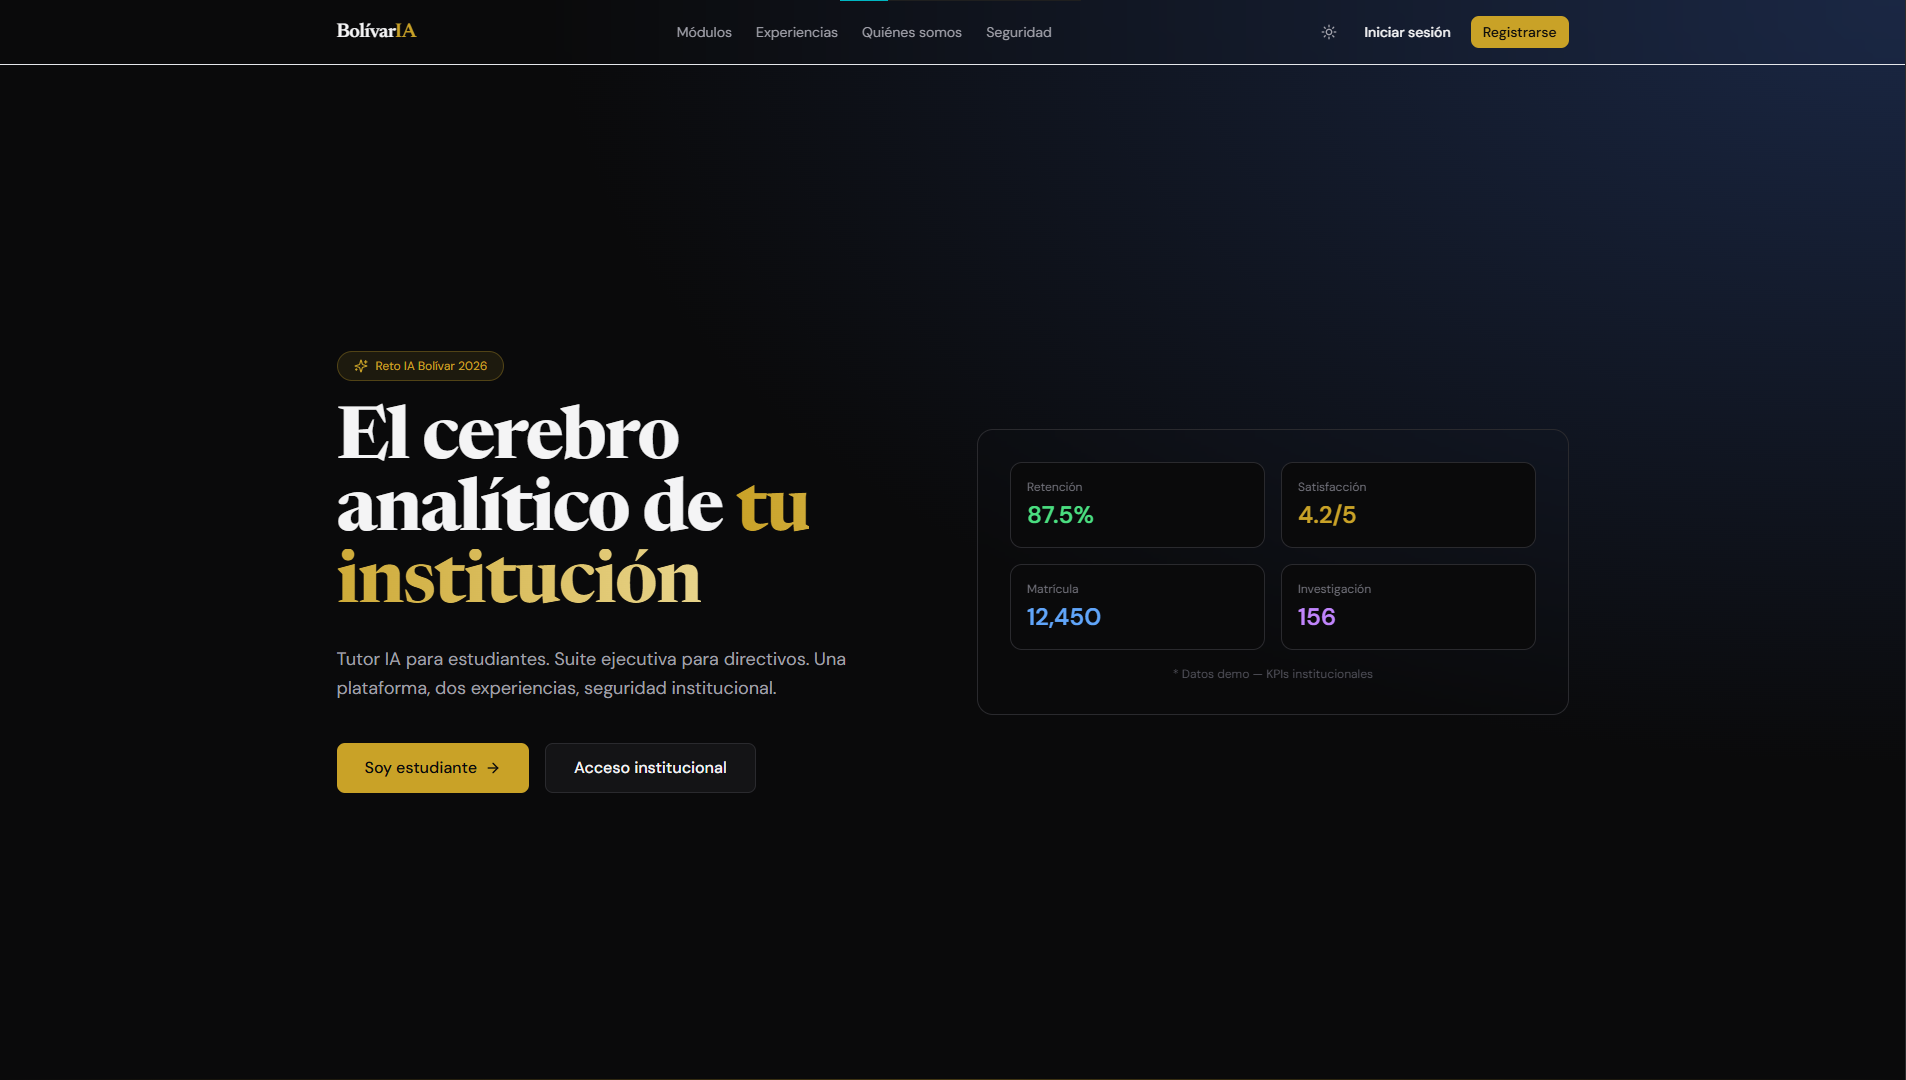
\includegraphics[width=\textwidth]{../img/imagen_1.png}
  \caption{Landing del prototipo. Los KPIs visibles están identificados en la
  aplicación como datos demo y no representan impacto medido.}
\end{figure}
\clearpage

\begin{figure}[ht]
  \centering
  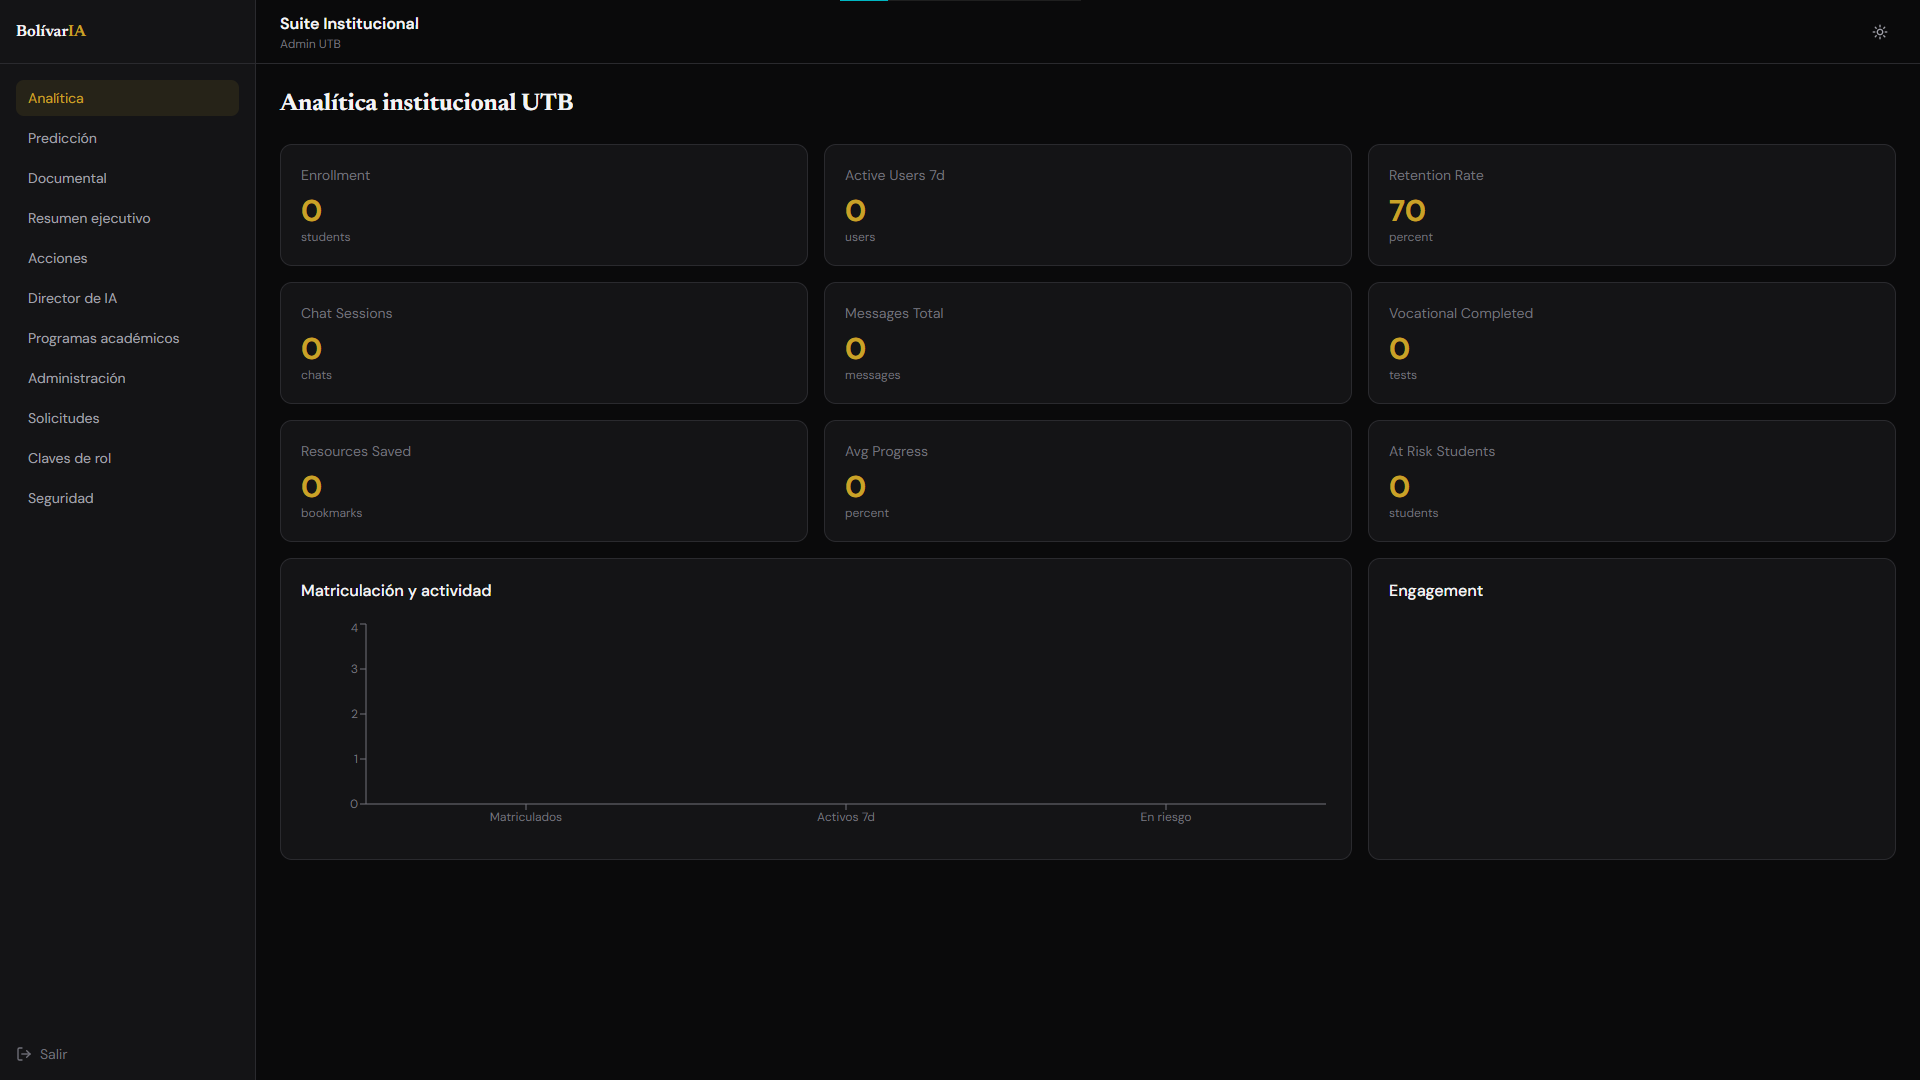
\includegraphics[width=\textwidth]{../img/imagen_4.png}
  \caption{Vista institucional del prototipo. La interfaz demuestra la
  estructura del tablero; los valores dependen de la carga de datos.}
\end{figure}
\clearpage

\section*{Conclusión}
\addcontentsline{toc}{section}{Conclusión}

UTB Te acompaña demuestra factibilidad técnica y un rediseño valioso del proceso
de acompañamiento: señales estructuradas, riesgo explicable, priorización y
supervisión humana. Su principal fortaleza no es reemplazar decisiones, sino
reducir el tiempo necesario para identificar y atender a quien necesita apoyo.

El siguiente hito no debe ser agregar más funcionalidades, sino validar el
circuito con datos y usuarios reales bajo autorización institucional. Un piloto
controlado permitirá reemplazar estimaciones por métricas, medir equidad y
precisión, confirmar el ROI y formalizar la gobernanza requerida para escalar.

\vfill
\begin{center}
  \color{utbblue}\rule{0.65\textwidth}{1pt}\\[3mm]
  \textbf{UTB Te acompaña}\\
  \small Universidad Tecnológica de Bolívar · Reto IA Bolívar 2026
\end{center}

\end{document}
